\documentclass{sig-alternate}
\graphicspath{{graphics/}}
\usepackage[hang]{subfigure}

\begin{document}

% --- Author Metadata here ---
%\conferenceinfo{WOODSTOCK}{'97 El Paso, Texas USA}
%\CopyrightYear{2009} % Allows default copyright year (200X) to be over-ridden - IF NEED BE.
%\crdata{0-12345-67-8/90/01}  % Allows default copyright data (0-89791-88-6/97/05) to be over-ridden - IF NEED BE.
% --- End of Author Metadata ---

\title{Adaption of XCS to predator/prey scenarios}
\subtitle{[Extended Abstract]}

\numberofauthors{3}
\author{
\alignauthor
Clemens Lode\\
       \affaddr{Karlsruhe Institute of Technology}\\
       \affaddr{Institute AIFB}\\
		 \affaddr{76128 Karlsruhe, Germany}\\
       \email{clemens@lode.de}
\alignauthor
Urban Richter\\
       \affaddr{Karlsruhe Institute of Technology}\\
       \affaddr{Institute AIFB}\\
		 \affaddr{76128 Karlsruhe, Germany}\\
       \email{urban.richter@kit.edu}
\alignauthor
Hartmut Schmeck\\
       \affaddr{Karlsruhe Institute of Technology}\\
       \affaddr{Institute AIFB}\\
		 \affaddr{76128 Karlsruhe, Germany}\\
       \email{hartmut.schmeck@kit.edu}}

\date{30 July 2009}

\maketitle



\begin{abstract}

This paper investigates an approach of concurrent learners, where the credit assignment problem is specially addressed (How to divide team reward among the individuals?). Moreover, the investigated approach is focussed on the dynamics of learning (How to cope with the problem of coadaptation?) in a scenario as an instance of the homogeneous and (non-) communicating predator/prey example. To compensate the dynamic nature of such a scenario a new algorithm is developed ("`SXCS"') by modelling the reward function according to an heuristic with high performance and by using memory to record the movements and the history of function's past values.

\end{abstract}


\section{Introduction}\label{section:introduction}

In this paper a predator/prey scenario~\cite{miller:1994:CPE} in the connection with a learning classifier system (LCS) is examined. Following the global task to observe one or up to $n$ (randomly) moving targets/preys, a number of rovers/predators has to achieve a common goal with local and distributed behavior, e.\,g., maximizing the global observation time or catching moving target(s). The scenario shows technical relevance to Organic Computing scenarios and it seems to be very flexible in its parameterization. Especially, it allows many variations: Depending on the playground the agents have to live in, implementations can vary the number of agents, the number of targets, the number and distribution of obstacles, the moving strategies, the learning behavior of the agents, the definition of local neighborhoods, the communication possibilities between the agents, and various forms of collaboration and collective learning could be analyzed. E.\,g., agents can learn strategies for any given group behavior and they can exchange locally learned knowledge -- to benefit from their swarming behavior or to adapt quicker than in a single-agent case. 

Thus, the challenge of concurrent learning agents is addressed, where all agents are equipped with a single, independent LCS. A current field of research in the field of LCS are the so-called \emph{eXtended Classifier Systems} (XCS)~\cite{Wil95}\cite{Butz2006}\cite{BW00}. Basically a XCS is a LCS, i.e. a number of rules, so-called \emph{classifiers}), each consisting of a condition and an action. When the sensors of an agent match to a condition then the action is executed. As wild-cards can be part of the condition a mechanism usually has to select from multiple classifiers. The classifiers are updated and adapted to the environment step by step using \emph{reinforcement learning}. When an agent reaches a goal condition a reward is distributed among the classifiers. The way this is done usually depends on the type of scenario, in a single-step environment a reward is generated at each step while in a multi-step environment with local information the agent has to construct the global information using multiple repetitions and steps.


It has been ascertained that neither the single-step nor the multi-step approach of XCS, can be used to learn a dynamic observation task as described above. While there are implementations to handle such scenarios, they are either very simple with a goal object that can only be moved by agents, with only one or two agents and no obstacles~\cite{1102281} or use global communication and organization with a shared global classifier set, for example in~\cite{TTS01}.

TODO mehr Quellen?
TODO profit sharing \cite{Miyazaki2} 


Thus, a promising modified XCS approach has been investigated to overcome the drawbacks of the classical XCS algorithm. The proposed idea is mainly based on a local cooperative reward function and some kind of temporary memory, which stores past actions sets and their corresponding reward values. Thus, local payoffs can be delayed and the reward function reflects in a better way the local agent behavior. Cooperation (incorporated in the reward function) is more or less achieved through rejection and attraction. Predators reject each other, the prey attracts the predators. Thus, agents try to uniformly distribute on the grid and observation time of the prey seems to be maximized. In addition it is shown that the new XCS approach retains its ability to recognize local obstacle configurations in order to reach the goal object.



\section{Learning Classifier Systems}
\label{section:learning-classifier-systems}

The field of learning classifier systems (LCSs), introduced in the 1970ies \cite{Hol75,Hol76,HR78}, is one of the most active and best-developed form of genetic based machine learning \cite{KL00,Kov02a,Lan08}. As mentioned above, much of learning classifier's theory is inherited from the reinforcement learning literature. The following section provides a brief overview what an LCS is. 

The architecture of an LCS is simple to study and the knowledge is encoded and stored in so-called \emph{classifiers}. These classifiers consist of a condition part, which is matched against the input from the environment, an action part (\emph{condition $\rightarrow$ action}), and some kind of fitness or strength value. The rule syntax is very simple and represents very fine-grained knowledge. This simple representation allows the LCS to use genetic operators for rule discovery.

The strength value is used to decide, which classifier should be chosen if more than one classifier matches the current input. The encoding of conditions is done in such a way that different levels of \emph{generality} are possible, hence the range of input values each classifier matches against may vary from a single point to the entire search space. In a step that is called \emph{rule discovery} new classifiers are generated using genetic operators, like crossover and mutation, on existing classifiers, changing both condition and action. Furthermore, every time no classifier matching the current input is available, one or more classifiers with a matching condition and randomly chosen action are created (this is called \emph{covering}).

After a classifier has been generated, the system has to determine its strength value. Every time a classifier's action is chosen, the strength value of this classifier is updated using some objective function. 

In certain problems (see section~\ref{subsection:single-step-vs-multi-step-problems}) the environment's reaction on some action executed by the LCS is not instantaneous, therefore the current value of the objective function is used to update the value of the classifier that was active during the \emph{previous} time step. 

The simplest way to increase performance would be to try and find classifiers, which maximize the objective function's value. Another approach more suitable for complex problems is the use of three distinct components as \emph{strength value}: The prediction $p$ of the objective function's value after this classifier's action has been executed, the average error of this prediction $\epsilon$, and a fitness value $F$ computed from this prediction error. The prediction is used to choose an action for execution: The classifier with best prediction, weighted by its fitness, is likely to result in best performance. Furthermore, the fitness is used to find classifiers suitable as input for the generation of new classifiers using genetic operators. The goal is to represent the entire search space with as few classifiers as possible while keeping only those that are more \emph{accurate} in their prediction. This approach is realized in \emph{XCS, the eXtended Classifier System} \cite{Wil95}, which is used within this paper and described in \cite{But00,BW00,BW02}.


\subsection{Single-Step vs. Multi-Step Problems}
\label{subsection:single-step-vs-multi-step-problems}

Literature about LCSs is divided into single-step and multi-step approaches. This separation bases on how to solve the reinforcement learning problem and addresses a design decision, which has to be taken when implementing an LCS. It refers to the question \emph{when} a reinforcement signal (reward) is achieved from the environment and \emph{how} this reward is distributed on the past action(s). 

In single-step environments the external reward is received on every time step and the environmental input for each time step has completely been independent of the prior time step in the case of environments with only a single entity with a LCS. When a decision is made, the reinforcement is directly received and measures the quality of the decision. Single-step environments generally involve categorization of data examples. A typical single-step benchmark problem is the \emph{boolean multiplexer problem} \cite{Wil95,BKLW04}. 

In multi-step environments the external reward may not necessarily be received on any time step, since the environmental input on a time step depends on at least the prior input and the system's last action. Typical multi-step environments are known as sequential environments or so-called \emph{Maze} problems, e.\,g., \emph{Wood1}~\cite{Wil94} or \emph{Wood2}~\cite{Wil95}. These examples model the adaptive interaction of an agent with its environment and have been studied using a variety of methods. Most often, a Maze is defined as a given number of neighboring cells in a grid-world. A cell is a bounded space formally defined and is the elementary unit of a Maze. When a cell is not empty, it can contain an obstacle, food, a so called \emph{animat}, and eventually a predator of the animat. 

An animat is randomly placed in the Maze environment (which could be some kind of a labyrinth) and it tries to set its position to a cell containing food, which is sparsely located in the environment. To perform this task, it possesses a limited perception of the environment. The animat's viewpoint is often limited to the eight cells surrounding the animat's position and it can also only move to an empty cell of this set of neighboring cells. Moving step by step through the Maze in order to fulfil its goal the animat searches for a strategy (or adopt a policy), which minimizes the effort undertaken to find the food in the selected Maze environment. 

Maze environments offer plenty of parameters that allow to evaluate the complexity of a given system and also to evaluate the efficiency of a learning method. A full description of these parameters is available in \cite{BZ05}.


\subsection{Non Markov environments}\label{subsection:nonmarkov_environments}

Some Maze problems offer perceptually similar situations that require different actions to reach the goal/food. This problem is often studied in the context of \emph{non Markov environments}. Woods101 (see fig.~\ref{figure:woods101}) is a typical example of a \emph{partially observable Markov decision process (POMDP)}, where a \emph{single-agent} cannot distinguish different situations due to a lack of global environmental information. The animat is placed in a free random field, it can sense the eight adjacent cells and has to learn to reach food while trees blocking any movement. Here the positions marked with 1 and 2 share the same sensory configuration so XCS cannot evolve an optimal policy for Woods101.

\begin{figure}[ht]
  \subfigure[The Woods101 environment with aliasing positions marked with 1 and 2]{
  	\label{figure:woods101a}
  	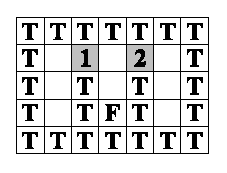
\includegraphics[width=0.25\textwidth]{woods101a.eps}}\hfill
  \subfigure[Sensory configuration of the two aliasing positions]{
  	\label{figure:woods101b}
  	
\includegraphics[width=0.15\textwidth]{woods101b.eps}}\hfill
  \caption{Trees are marked with T, food is marked with F. The aliasing positions in fig.~\ref{figure:woods101a} share the same sensory configuration (see fig.~\ref{figure:woods101b}), but require different optimal actions.}
  \label{figure:woods101}
\end{figure}


Using records of past situations/actions by adding temporary memory is a
widespread approach to cope with such environments, as investigated in
\cite{Lan98,LW00}.

A second non Markov property is still embedded in \emph{multi-agent} environments and this is related to a change of an agent's internal state. In scenarios with more than one learning agent, an agent has to evaluate actions that may be caused by its own internal state or that are the result of other agent's actions. It is difficult to recognize an environmental change, which is caused by the change of another agent's internal state, due to a lack of the other agents' information. Even if an agent stays in the same location the agent cannot evaluate the environmental changes. In \cite{TTS01}, this second non Markov property is defined as the \emph{non observable Markov decision process (NOMDP)}. Thus, since multi-agent scenarios often include both non Markov properties (POMDP and NOMDP), learning in multi-agent environments is more complex than learning in single-agent environments. 


\section{Scenario}\label{section:scenario}


TODO �berleitung, Reihenfolge der Unterpunkte
TODO Bezeichnung environment/scenario

The algorithms are tested in a simple predator/prey scenario on a torus with discrete squares. The field is a quadrat consisting of 16x16 squares. The prey consists of a single moving goal object which the predators (the agents) have not to catch but to keep under surveillance. The quality of an algorithm that controls the agents is determined by the share of the time any agent has the goal object in surveillance range. It is calculated by averaging the qualities of 10 problems per experiment and 10 experiments. In each time step each agent can move only to one of the four neighboring fields while the goal object can move two fields. In addition there are obstacles on the field and any movement to an occupied field fails (without any further consequences). Both the goal object and the agents have 12 binary sensors that can sense their close environment (up to two fields distance) while another 12 binary sensors can sense the environment further away (up to five fields distance), see Fig.~\ref{figure:sight_directions}. The 12 sensors are for the four directions and the three types of objects (goal object, other agents and the obstacles). Obstacles do block the lines of sight of a sensor.


\begin{figure}[ht]
\centerline{	
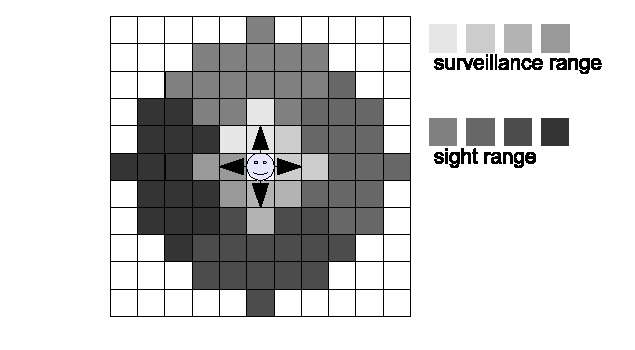
\includegraphics[width=0.4\textwidth]{sight_directions.eps}
}
\caption{Sight range ($5.0$, dark area) and surveillance range ($2.0$, bright area) of an agent / the goal object for each direction}
\label{figure:sight_directions}
\end{figure}

The simulation is conducted in discrete time. At every time step the goal object and the agents gather sensor data and decide their next actions. Then all actions of all objects are executed in a random sequence. As the goal object can move two fields it gathers new sensor data after the first step. If the goal object is surrounded by agents in all 4 directions it jumps to a random nearby free field which basically means a restart of the simulation. Experiments showed that this happened in a few cases, so it does not affect the result.


\subsection{The Predator/Prey Example}
\label{subsection:the-predator-prey-example}

As an example of a multi-agent approach, the predator/prey domain is an appropriate example that has successfully been studied in a variety of instantiations. It does not serve as a complex real world domain, but as a test scenario for demonstrating and evaluating manifold research ideas. Introduced by \cite{BJD86}, researchers have investigated different instantiations of its original formulation in the context of different application areas. 

Both, predator and prey, typically can move into four different directions -- north, east, south, and west. Mostly, predators follow a capturing strategy as a goal, while the prey randomly moves or stays still with a certain probability in order to simulate slower movements than the predators. A variation is that the prey moves faster than the predators. In this case a strategic collaborative effort is required by the predators. An active escaping strategy where the prey adapts and learns its behavior may also be possible.

A cell of the two-dimensional grid-world can only be occupied by one agent.
Worlds with other shapes as spaces (e.\,g., squares) or continuous/toroidal
worlds without edges (predators and prey can move off one end of the world
and come back on another end) are possible. 

The predators try to capture the prey in such a way that the prey cannot move to an unoccupied position. If the grid world has edges, it might be possible that fewer than four predators can catch the prey by surrounding the prey against an edge of obstacles or in a corner of the world. Other parameters of the predator/prey domain are: Do the agents move simultaneously or successively -- one after the other? Is the local view of an agent limited or does an agent see the whole environment? And last, but not least, is direct communication between the agents allowed?

While predators and prey(s) have limited actions and follow well defined objectives, the predator/prey domain is simple to understand, easy to implement, and flexible enough to demonstrate a range of different scenarios, which have been emerged over the past decades. The general approach of the predator/prey example, the possibility to customize and adopt the scenario to manifold applications, or the widespread experience that is documented, not only in multi-agent literature, result in the assumption that the predator/prey example can be used as a valid testbed for OC scenarios.

TODO mit tats�chlich verwendeten Szenario verkn�pfen, evtl subsection weiter hoch schieben


\subsection{Scenario configurations}

Three different configurations of obstacles and starting positions of the agents and the goal object were thoroughly tested. All configurations consisted of a 16x16 torus grid with obstacles and 8 agents. In the \emph{pillar scenario} (see fig.~\ref{figure:pillar_scenario}) there were 4 obstacles in equal distance to each other, with the goal object starting in the center and the agents starting randomly along the borders. The idea was to minimize the number of blocked fields while still giving the agents some points of orientation.
In the second scenario, the \emph{random scenario}, several obstacles were placed randomly on the field, with a certain tendency to build connected structures. The third scenario consisted of a cylinder and several walls with small openings. There, the goal was to find those openings that lead to the goal object which always stayed in the last section.

\begin{figure}[ht]
  \subfigure[Pillar scenario]{
  	\label{figure:pillar_scenario}
   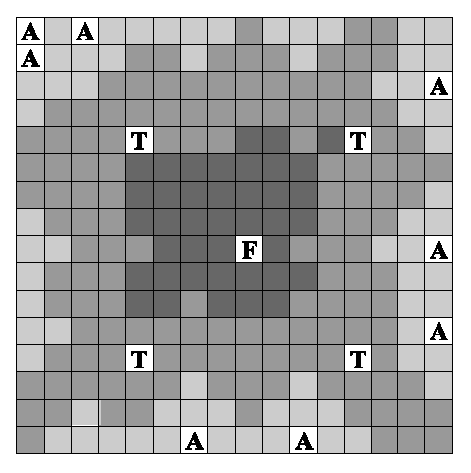
\includegraphics[width=0.14\textwidth]{testpillar.eps}
  }\hfill
  \subfigure[Random scenario]{
  	\label{figure:random_scenario}
  	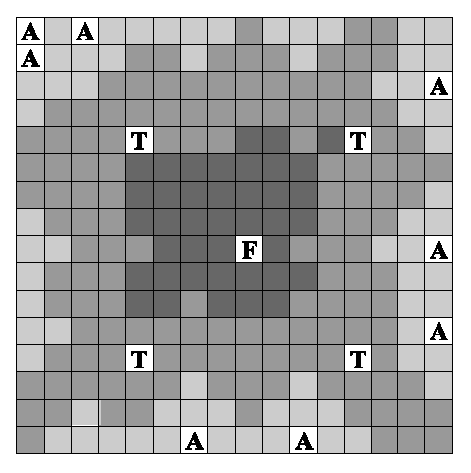
\includegraphics[width=0.14\textwidth]{testpillar.eps}
  }\hfill
  \subfigure[Difficult scenario]{
  	\label{figure:difficult_scenario}
  	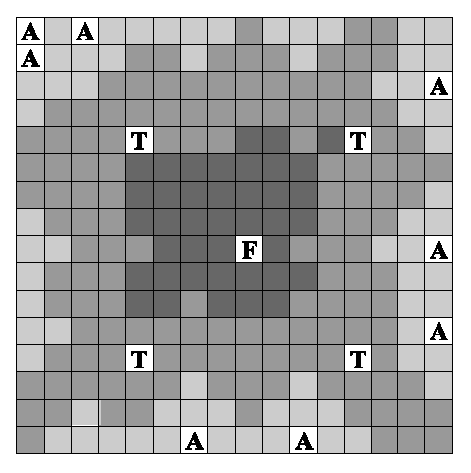
\includegraphics[width=0.14\textwidth]{testpillar.eps}
  }

  \caption{These are sample start configurations for the three different types of scenarios. Trees are marked with T, food is marked with F, agents are marked with A and the surveillance and sight range is marked with light and dark grey color.}
  \label{figure:scenarios}
\end{figure}


\subsection{Classification of the scenario}

As described in section~\ref{subsection:nonmarkov_environments} environments can be classified as a MDP, a POMDP or a NOMDP. The main characteristics of a predator/prey scenario are:

\begin{enumerate}
\item An agent has only access to local information,
\item the field usually consists of open areas with randomly placed obstacles,
\item agents each have an internal state unknown to other agents,
\item the scenario is dynamic,
\item the agents are sharing a global goal and
\item the scenario runs continuously.
\end{enumerate}

Clearly the scenarios in question constitute no MDP because of limited sensory information (1, 3) and many different positions sharing the same sensory configuration (2). As the introduction of memory would not restore the Markov property (4) it is not a POMDP either. This leaves the scenario as being a NOMDP. In addition special care is needed when applying XCS as is no clear local goal (5) and the scenario is not restarted when reaching the global goal (6). All in all this means that a different approach is needed and a new XCS variant needs to be created that can handle these issues properly.

In the literature NOMDP environments are discussed in connection with XCS~\cite{TTS01,Miyazaki2}. There, the issue of non observability is either evaded by a very simple scenario with only two agents or solved by using very complex communication and central organization where the agents share a classifier system. Neither approach can be used here as the scenario is rather complex with many agents and there is no communication between the agents allowed. Thus, the first step is to look into the prerequisites of the algorithm of the usual XCS and then develop it further in order to be applicable to such a dynamic collaborative scenario.


\subsection{Learning in an environment with Markov property}

When the environment in question does have the Markov property then an agent can acquire global information through repetition of the same problem. When the goal is reached the scenario is restarted and the last action is evaluated positively. Actions that were executed before that last action that reached the goals are evaluated positively as well. By this way an optimal route can be found after a large enough number of cycles.

Usually an experiment runs either in an \emph{explore} or an \emph{exploit} phase. In the \emph{explore} phase classifiers are selected randomly in order to cover the search space while in the \emph{exploit} phase the performance is measured and classifiers are selected by the product of their fitness and prediction values.

TODO surveillance scenario nennen
TODO Subsection in Zusammenhang setzen oder raus


\section{Adaption of XCS to the scenario}\label{section:adaption_of_xcs}

In order to compare a new algorithm to XCS it is required to make the following adaptions to the standard implementation of XCS:

\begin{itemize} 

\item The performance is tested at all time and not only during \emph{exploit} phases,
\item the reward function has to be adjusted to the fact that there is no distinct goal to reach and that the quality of an algorithm is determined by constant good behavior (see section~\ref{subsection:reward_function}),
\item besides the usual goal condition "`goal found"' with a positive reward there will also be a goal condition "`goal lost"' with a reward of zero (see section~\ref{subsection:events}),
\item some XCS parameter were adapted (see section~\ref{subsection:parameter}),
\item the problem always runs 2,000 time steps and is not reset when some condition occurs as the scenario demands a continuous observation of the goal object and
\item the genetic operator uses two fixed locations for the \emph{two point crossover} because of the way sensory data is acquired.

\end{itemize}


\subsection{Reward function}\label{subsection:reward_function}

In a single-step environment the optimal representation of the reward function by the XCS is also the solution of the actual problem. For example in the 6-multiplexer problem the reward function already contains the table of the 6-multiplexer itself. The main prerequisite of an environment that can be solved by the single-step method is that the agent has global information. More complex problems that do not satisfy this prerequisite, i.e. problems where the agent only has local information, need to be solved by building up global information out of a sequence of local information parts. In order to accomplish this the agent must be able to distinguish between all positions, i.e. the scenario has to have the Markov property.



In the standard implementation of XCS there is very much time available and that by resetting the scenario and repeating the same steps in the same local environment it is possible to reach the goal. On the other hand, in a dynamic environment the global information cannot be constructed as in the time the information is gathered it is no longer valid because other agents and the goal object may have moved. Also, the scenario cannot be repeated expecting the same behavior of the environment. Thus it is important to speed up the learning and connect the learning steps directly instead of gradually pass the reward down.

The actual reward function in the multi-step environment often consists of a simple binary value that is determined by the position of the agent compared to the goal position, i.e. whether it has reached the goal or not. In the predator/prey scenario the nature of the reward function is not obvious. 

As the reward function runs locally on each agent and as the reward that it calculates depends on the sensor data, basically an agent has free choice about how this function should look like. 24 binary sensors result in up to \(2^{24}\) situations an agent can recognize (actually \(3^{12}\) due to some redundancy) and an equal number of reward functions if each situation is assigned an own value. This surpasses the available memory. 

To answer the question one need to look at the global goal. One possibility is to choose a reward function by testing heuristics. Although heuristics do not work with a reward function as they do not learn it still evaluates situations and corresponding actions either as "`good"' ("`move in that direction"') or as "`bad"' ("`don't move in that direction"').

Of a set of simple implementations the best results delivered the following heuristic:

\begin{itemize}
\item If the goal object is not in sight: Move randomly in a direction without other agents in sight
\item Otherwise: Move in the direction of the goal object
\end{itemize}


In this implementation a binary reward function was used. This causes some problems when trying to model the heuristic as it is impossible to distinguish situation with e.g. one other agent and four other agent in sight. Probably a better implementation would be to count the number of agents and return it as a reward. An additional problem surfaces in scenarios with a relatively low number of agents because the reward function returns 1 most of the time. This could harm the learning process.

As further adaptions to the reward is necessary the value the reward function returns will be called "`base reward"'. Below (section~\ref{subsection:events}) the actual reward for the rules of the XCS will be calculated.

\begin{figure}[ht]
\setbox0\vbox{\small
Model of the reward function:
\begin{itemize}
\item Goal object not in sight, at least one other agent in sight \(\Rightarrow\) \emph{base reward}~\( = 0\),
\item Goal object not in sight, no other agent in sight \(\Rightarrow\) \emph{base reward}~\( = 1\) and
\item Goal object in sight \(\Rightarrow\) \emph{base reward}~\( = 1\).
\end{itemize}
}
\centerline{\fbox{\box0}}
\end{figure}


\subsection{Events}\label{subsection:events}

Compared to the usual implementation in~\cite{BW00} the main difference is that the environment does not restart when it returns a positive reward. That is because the goal is not only to get the goal object in sight but to keep it there.

Assuming that the agent did something right when it comes into sight range of the goal object (or leaving the sight range of all other agents) such a situation change will be called a "`positive event"' while loosing the goal object or getting into sight range of other agents will be called a "`negative event"'. Thus a positive event occurs whenever the base reward changes from 0 to 1, a negative event occurs whenever the base reward changes from 1 to 0. 

As there can be cases where an agent never encounters an event the number of steps is limited to \emph{maxStackSize} steps. If that number is reached then a "`neutral event"' occurs. This means that the step number is reset to 0 and the classifier system waits for a new event.


\subsection{Reward distribution}\label{subsection:reward_distribution}

The standard implementation of XCS is based on the assumption that it works in an environment with the Markov property. This is expressed in the way the reward is distributed between the classifiers that contributed to reaching the goal. It requires several repetitions in order for the reward to be transferred to all classifiers that contributed to the solution.

In the dynamic predator/prey scenario such repetitions are not available, the scenario is not restarted and runs continuously. This is the reason why separate measures have to be taken in order to reward previous contributing steps as well.

In the new XCS variant SXCS (\emph{Supervising eXtended Classifier System}) that is presented here not only the last action step but all past action sets will be recorded. Such a memory mechanism does not restore the Markov property because the scenario is a non observable Markov decision process. But it does restore the connection of the reward between the goal and previous contributing steps and an improvement in the performance is to be expected.


\subsection{Implementation of SXCS}\label{subsection:sxcs_implementation}

Whenever (and only then) an event occurs the reward is distributed among the entries of the action sets that were saved since the last event. This is done with a quadratic function, i.e. with \(r(a)\) being the \emph{reward} for the \emph{action set} with age \(a\):
$$
r(a) = \left\{ \begin{array}{rl}
  \frac{{a}^{2}}{{\mathrm{size(\emph{action set})}}^{2}} &\mbox{ \emph{positive event}} \\
  \frac{{(1 - a)}^{2}}{{\mathrm{size(\emph{action set})}}^{2}} &\mbox{ \emph{negative event}} \\
  1 &\mbox{ \emph{neutral event}, \emph{base reward} = $1$} \\
  0 &\mbox{ \emph{neutral event}, \emph{base reward} = $0$}
       \end{array} \right.
$$

The idea behind using a quadratic function is that it loosely resembles the transfer of the reward in the original implementation. Other implementations are possible, this is merely the simplest approach. An example is shown in fig.~\ref{figure:saved_rewards}, for simplicity a linear distribution was used, in the tests no significant difference was observed when comparing linear distribution with quadratic distribution.

\begin{figure}[ht]
\centerline{	
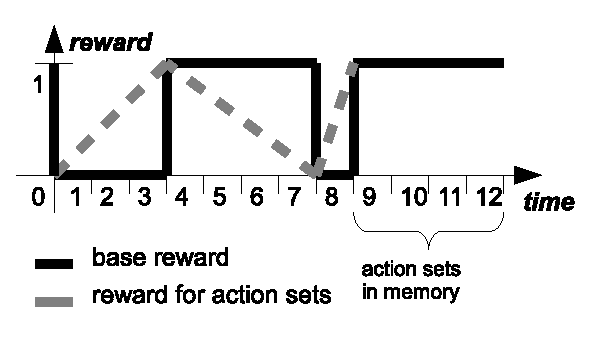
\includegraphics[scale=0.75]{saved_rewards.eps}
}
\caption{Schematic presentation of the reward distribution to the action sets over time after several positive and negative events}
\label{figure:saved_rewards}
\end{figure}


There are two drawbacks with this implementation: Firstly there is a time delay of the reward distribution because it is impossible to foresee when an event will occur. Secondly, in the case of a neutral event, the prediction of future events could be wrong and a new positive or negative event occurs shortly after the neutral event (see fig.~\ref{figure:neutral_reward}). Both points do not seem significant because the time delay, compared to the standard implementation with repetition of the problem, is very small and the erroneous reward distribution in the case of a neutral event could be corrected retroactively to a certain degree. On the other hand recording the history of rewards could provide a basis for a deeper analysis resulting in a better reward distribution than the one that is presented here.

% zeigt die Bewertung bei einem solchen neutralen Ereignis, bei dem nach einem �berlauf die erste H�lfte mit \(1\) bewertet wurde. Au�erdem ist dort der maximale Fehler dargestellt, welcher eintreten w�rde, wenn direkt beim Schritt nach dem Abbruch eine �nderung des \emph{base reward} Werts auftritt. Im dargestellten Fall w�rde sich also der \emph{base reward} Wert beim aktuellen Zeitpunkt auf \(0\) ver�ndern.\\


\begin{figure}[ht]
\centerline{	
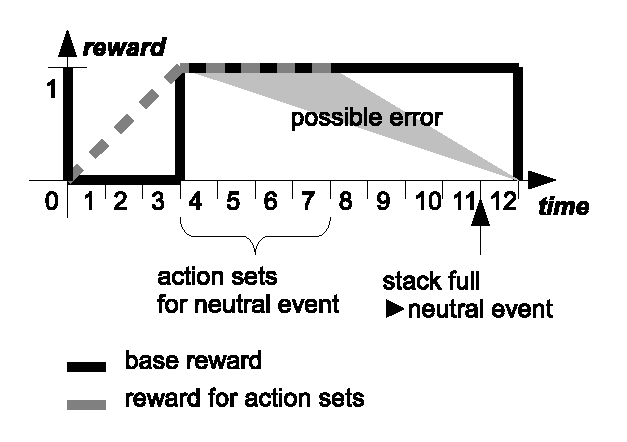
\includegraphics[scale=0.75]{neutral_reward.eps}
}
\caption{Schematic display of the reward distribution to the action sets after a neutral event (with \emph{base reward} = 1)}
\label{figure:neutral_reward}
\end{figure}


%In XCS wird lediglich die jeweils letzte \emph{action set} Liste aus dem vorherigen Schritt gespeichert. In der neuen Implementierung werden dagegen eine ganze Anzahl (bis zum Wert \emph{maxStackSize}) von \emph{action set} Listen gespeichert. Die Speicherung erlaubt zum einen eine Vorverarbeitung des \emph{reward} Werts anhand der vergangenen Schritte und auf Basis einer gr��eren Zahl von \emph{action set} Listen und zum anderen die zeitliche Relativierung einer \emph{action set} Liste zu einem Ereignis. Die \emph{classifier} werden dann jeweils r�ckwirkend anhand des jeweiligen \emph{reward} Werts aktualisiert, sobald bestimmte Bedingungen eingetreten sind.\\

%Bei der Benutzung eines solchen Stacks entsteht eine Zeitverz�gerung, d.h. die \emph{classifier} erhalten jeweils Informationen, die bis zu \emph{maxStackSize} Schritten zu alt sein k�nnen. Tritt beim Stack ein �berlauf auf, gab es also \emph{maxStackSize} Schritte lang keine �nderung des \emph{base reward} Werts mehr, dann wird abgebrochen und die \(\frac{maxStackSize}{2}\) �ltesten Eintr�ge werden vom Stack genommen. Alle diese Eintr�ge werden dabei vorher mit einem \emph{reward} Wert aktualisiert, der diesem \emph{base reward} Wert entspricht.\\

%In such a case 


\begin{figure}[ht]
\setbox0\vbox{\small
All in all an event occurs when...
\begin{itemize}
\item the \emph{base reward} changes from 0 to 1 (goal object entered and/or the last agent left the sight range) \(\Rightarrow\) {\bf positive event},
\item the \emph{base reward} changes from 1 to 0 (goal object left and/or the first agent entered the sight range) \(\Rightarrow\) {\bf negative event},
\item there is a stack overflow (no positive or negative event in the last \emph{maxStackSize} steps) and the goal object is in sight range and/or no agents are in sight range \(\Rightarrow\) {\bf neutral event} (with \emph{base reward} = \(1\)) or when
\item there is a stack overflow (no positive or negative event in the last \emph{maxStackSize} steps) and the goal object is not in sight range and/or an agent is in sight range \(\Rightarrow\) {\bf neutral event} (with \emph{base reward} = \(0\)).
\end{itemize}
}
\centerline{\fbox{\box0}}
\end{figure}



\subsection{Size of the stack (\emph{maxStackSize})}\label{subsection:sxcs_stack_size}

An open question is the size of the stack. In this paper a good value was determined by tests, further research is needed in that direction. It is needed to find a compromise between three conflicting factors. Large values can lead to a delay between the rewarding situation and the actual reward and the reward of uninvolved rules. On the other hand, small values can lead to early stack overflows and a possible disregard of rules that are crucial to solve the problem.

As fig.~\ref{figure:max_stack_size} shows the value does not have a large impact, only at around \emph{maxStackSize}~\( = 8\) a difference can be seen. Other tested scenarios favor larger values so the value is scenario dependant.

\begin{figure}[ht]
\centerline{	
%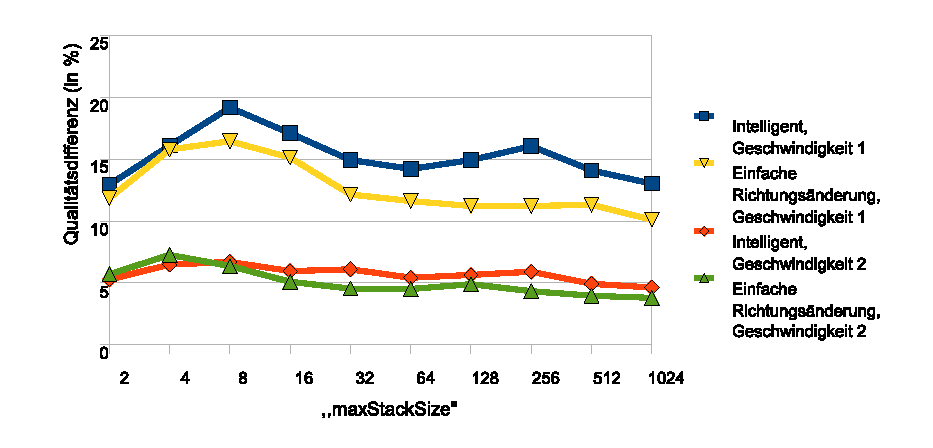
\includegraphics{max_stack_size.eps}
}
\caption{Comparison of different values of \emph{maxStackSize} in various scenarios}
\label{figure:max_stack_size}
\end{figure}




\subsection{XCS Parameter}\label{subsection:parameter}

Most of the parameters correspond to the standard values given in~\cite{BW00} ("`Commonly Used Parameter Settings"'). Below special settings are discussed. While thousands of different combinations were tested, the parameter discussion is not necessarily complete. Of main importance was that any score below the algorithm where the agents move randomly has to be dismissed as it is difficult to say if a parameter settings with better results (below the result of the random algorithm) just makes the agent move more randomly or if it actually learns better.

According to~\cite{BW00} the maximum number of classifiers \(N\) should be chosen big enough so that \emph{covering} happens only in the beginning of a run. For the scenario in question tests have shown that a population size of around 512 fulfills this criteria. Although random initializations are possible (see~\cite{Butz2006}), it was chosen to start with empty classifier sets as tests have shown some advantages. The \emph{GA threshold} parameter $\theta_{\mathrm{GA}}$ was set to 25, larger values seemed to reduce the quality of the algorithm.
The parameter \emph{reward prediction discount} $\gamma$ is only needed to compare XCS with SXCS, SXCS itself does use quadratic reward distribution. Tests showed inconclusive results so the standard value of \(\gamma = 0,71\) was used. Only \(\gamma = 1,0\) showed significant different results, so it seems that while the reduction of the transfer of the reward is needed, the actual value is of little importance.


\subsection{Learning rate $\beta$}\label{subsection:learning_rate}

For the learning rate $\beta$ in a similar type of scenario in~\cite{1102281} a value below the standard value was proposed (\(\beta = 0,02\)). The reason was that dynamic multi-agent systems can be described only by movement probabilities so the learning process has to be slow and careful. In tests (see fig.~\ref{figure:pillar_learning_rate_quality}) an optimal value between \(0,01\) and \(0,1\) for SXCS was determined, larger values seem to harm the learn process significantly. For XCS on the other hand the quality increases with larger values for \(\beta\) in this scenario. This is still a subject of research, but because larger values result in loss of comparability with other implementations of XCS the standard value of \(0,2\) was used.

%TODO schwieriges Szenario

\begin{figure}[ht]
\centerline{	
%\includegraphics{lernrate_beta.eps}
}
\caption{Influence of the learning rate parameter $\beta$ on the performance (pillar scenario with XCS and SXCS agents and \emph{best selection})}
\label{figure:pillar_learning_rate_quality}
\end{figure}


%TODO pruefen ob notwendig 
%~\cite{subsection:tournament_factor_test}

\begin{table}[ht]
\caption{Used parameter values and standard values}
\centering
\begin{tabular}{c c c}
\hline\hline
Parameter & Value & Standard~\cite{BW00}\\ [0.5ex]
\hline
max population \(N\) & \textbf{512} & [-]\\
subsumption threshold \(\theta_{\mathrm{sub}}\) & 20,0 & [20,0+]\\
GA threshold \(\theta_{\mathrm{GA}}\) & 25 & [25-50]\\
mutation probability \(\mu\) & \(0,05\) & [0,01-0,05]\\
reward prediction discount \(\gamma\) & 0,71 & [0,71]\\
learning rate \(\beta\) & \textbf{0,01 - 0,2} & [0,1-0,2]\\
tournament factor & 0,84 & [-]\\ [0.5ex]
\hline
\end{tabular}
\label{table:lcs_parameter}
\end{table}




\subsection{Implementation}

While it is possible to implement the idea of events in the original implementation as part of the environment by ignoring restart instructions, it would also have to handle the events which requires to save previous rewards for each agent. That is why it seemed more straightforward to rewrite the portion where the reward is evaluated and collected. Putting all together this results in the following modified version of the XCS algorithm. 
 
TODO source code


\section{Experiments}\label{section:experiments}

\subsection{Experiments with heuristics}\label{subsection:experiments_heuristics}
TODO
\subsection{Difficult scenario}\label{subsection:xcs_difficult_scenario}
TODO


\section{Conclusions}\label{section:conclusions}

TODO Text

All in all the results of this paper are:

TODO erst am Schlu� :)

\begin{itemize}

\item A good local evaluation function for the XCS can be constructed on the base of a heuristic with good performance (see section~\ref{subsection:reward_function}).

\item By adding external memory that records the reward history (see section~\ref{subsection:sxcs_implementation}) the newly created algorithm SXCS can solve the problem much better than XCS (see section~\ref{section:experiments}).

\item A variation of the learning rate $\beta$ can be successful depending on the scenario (see section~\ref{subsection:learning_rate} and section~\ref{subsection:xcs_difficult_scenario} for the difficult scenario respectively).

%\item Die Agenten mit XCS und SXCS haben deutliche Probleme mit Szenarien mit vielen Hindernissen (siehe Kapitel~\ref{subsection:tournament_factor_test}). TODO

%\item Ein dynamischer Wechsel der Auswahlart f�r Aktionen w�hrend eines Laufs kann sinnvoll sein, um die Zahl der blockierten Bewegungen zu verringern und das Zielobjekt besser verfolgen zu k�nnen (siehe Kapitel~\ref{subsection:analysis_random_scenario_xcs}). TODO

\item XCS as well as SXCS can solve difficult scenarios with positions of interest significantly better than randomly moving agents. Under certain circumstances SXCS can solve this scenario even better than the heuristic on which its evaluation function is based on (see section~\ref{subsection:xcs_difficult_scenario}).

\end{itemize}



\bibliographystyle{abbrv}
\bibliography{sigproc}


\end{document}
